\documentclass[11pt]{article}
% Libraries.

\usepackage{dsfont}
\usepackage{amsmath}
\usepackage{amssymb}
\usepackage{esint}
\usepackage[margin=2cm]{geometry}
%\usepackage{pgfplots}
\usepackage{graphicx}
\usepackage{enumitem}
\usepackage{hyperref}
\usepackage{fancyhdr}
\usepackage{perpage}
\usepackage[dvipsnames, pdftex]{xcolor}
\usepackage{float}
\usepackage{xargs}
\usepackage{/Users/raina/Desktop/uoft-notes/raina}
\usepackage[
	colorinlistoftodos,
	prependcaption,
	textsize=tiny
]{todonotes}

\numberwithin{equation}{section}

% Property settings.
\MakePerPage{footnote}
\pagestyle{headings}

% Attr.
\title{STA452\\ Lecture Notes}
\author{Yuchen Wang}
\date{\today}

\begin{document}
    \maketitle
    \tableofcontents
    \newpage
\section{Preface}
In our course, you will not see very much data. Our job is to express the ideas that drive the logic (or the logic that drives the ideas). As a consequence, the most of the examples in elementary book appear as pure theory. But they are not defined, they are consequences of abstract mathematical ideas.
For example, conditional density is a consequence of conditional expectation, which is an orthogonal projection in a vector space, a pure euclidean geometric idea.

\subsection{Preliminary}
\definition
A sequence of sets $A_n \rightarrow A$ iff $I(A_n) \rightarrow I(A)$.
%\remark
%	\red{See Appendix 2 of the original notes.}

\proposition A limit exists when the limsup is equal to the liminf:
\begin{equation}
	lim = \overline{lim} = \under{lim}
\end{equation}
\begin{proof}
For $w \in \Omega$,
	\begin{align}
		\sup_{t \in T} I(A_t)(w) &= I(\cup_{t\in T} A_t)(w) \\
		&= 1 \text{ or } 0 \\
		\inf_{t \in T} I(A_t)(w) &= I(\cap_{t\in T} A_t)(w)
	\end{align}
Therefore,
\begin{align}
	\lim_{n \rightarrow \infty} I(A_n) &= \underset{n \rightarrow \infty}{\overline{\lim}} I(A_n) \\
	&= \inf_{n=1}^\infty \sup_{k=n}^\infty I(A_k) \\
	&= I\left(\cap_{n=1}^\infty \cup_{k=n}^\infty A_k \right) \\
	&= \underset{n \rightarrow \infty}{\under{\lim}} I(A_n) \\
	&= \sup_{n=1}^\infty \inf_{k=n}^\infty I(A_k) \\
	&= I\left(\cup_{n=1}^\infty \cap_{k=n}^\infty A_k \right)
\end{align}
\end{proof}
\property Therefore it is clear that
\begin{enumerate}
	\item \begin{equation}
	A_n \rightarrow A \iff A = \cap_{n=1}^\infty \cup_{k=n}^\infty A_k = \cup_{n=1}^\infty \cap_{k=n}^\infty A_k
\end{equation}
	\item 
	\begin{equation} \label{monotone sequence limit 1}
		A_n \uparrow \implies A_n \uparrow \cup_{n=1}^\infty A_n
	\end{equation}
	\item
	\begin{equation} \label{monotone sequence limit 2}
		A_n \downarrow \implies A_n \downarrow \cap_{n=1}^\infty A_n
	\end{equation}

\end{enumerate}

\section{Virtual Dice}
\subsection{The Law of Large Numbers}
Consider a \ti{mechanism/process/system}, $W$, which generates \ti{outcomes}, $w$, in a sample space $\Omega$:
$$W: w_1, w_2, \hdots, w_n, \hdots$$
The outcomes are often referred to as \ti{trials} of the \ti{process} $W$. $w_n$ is called the $n$th trial, and the finite sequence ($w_1, w_2, 
\hdots, w_n$) is the first $n$ trials. \\
Consider any real-valued function $g: \Omega \rightarrow \real$ defined on the \ti{sample space} $\Omega$. Let $X = g(W)$ denote the \ti{extended process} that applies the function $g$ to the outcome $w$ from $W$ to produce the outcome $x = g(w)$. This new process has its own sequence of trial outcomes:
\begin{align}
	& g(W): g(w_1), g(w_2), \hdots, g(w_n), \hdots \\
    \text{or} \quad & X \quad \,\,\,  : x_1, x_2, \hdots, x_n, \hdots
\end{align}
These transformed outcomes are all real values, with which we can do lots of easy arithmetic, while the abstract sample space $\Omega$ may not have this property.
\definition[sample mean]
For each $n \in \mb{N}$, the \ti{sample mean} over the first $n$ trials is the \ti{arithmetic average} of the function values over those $n$ trials:
\begin{align}
	\widehat{E}_nX := \frac{g(w_1) + \hdots + g(w_n)}{n} = \bar{x}_n
\end{align}

\definition[random variable] A given process $W$ is said to be a \ti{random process / random variable} iff it satisfies the \ti{empirical law of large numbers}, in that, for any real-valued $X = g(W)$, we have
\begin{enumerate}
	\item \ti{stability}: the sequence of \ti{sample averages} ($\widehat{E}_ng(W), n \in \mb{N}$) converges;
	\item \ti{invariance}: the limit is independent of any particular realization ($w_n, n \in \mb{N}$).
\end{enumerate}

\definition[expected value]
For each real-valued $X = g(W)$, we obtain a \ti{expected value} in the above limit:
\begin{align}
	EX := \lim_{n \rightarrow \infty} \widehat{E}_n g(W) = \lim_{n \rightarrow \infty} \hat{x}_n
\end{align}
\definition[indicator function] The indicator function of a subset $A$ of a set $X$ is a function $I_A: X \rightarrow \{0, 1\}$ defined as
\begin{equation}
	I_A(x) := \begin{cases}
		1 & x \in A\\
		0 & x \notin A
	\end{cases}
\end{equation}
\definition[probability]
Now \ti{probability} itself is a special case of an \ti{expected value}: for any \ti{indicator function} $g = I_A$ with $A \subset \Omega$ we will get the usual sequence of averages, but now to be referred to as \ti{empirical relative frequencies}. These averages give the proportion of times that $A$ occurs in the first $n$ trials.
\begin{equation}
	\widehat{P}_n(W \in A) := \widehat{E}_n I_A(W) = \frac{I_A(w_1) + \hdots + I_A(w_n)}{n} \, \forall n \in \mb{N}
\end{equation}
As $n \rightarrow \infty$, the above equation gives the \ti{long-run frequency}, or \ti{probability}:
\begin{equation}
	P_W(A) = P(W \in A) := \lim_{n \rightarrow \infty}\widehat{E}_n I_A(W) = \lim_{n \rightarrow \infty}\widehat{P}_n (W \in A)
\end{equation}
\notation Given a random variable $W$ and a \ti{probability distribution} $P_W$, we can use the following notation:
$$W \sim P_W \quad \text{on} \quad \Omega$$
to be read as ``$W$ is distributed as $P_W$ on $\Omega$" or ``$W$ is distributed as $P_W$".

\subsection{Some examples: ``virtual dice"}
\definition \label{physical} For any specific $n \in \mb{N}$, the random variable $X$ is said to have a \ti{(finite discrete) uniform distribution} on the sample space $\Omega = \{1, \hdots, n\}$ (denoted $X \sim unif\{1, \hdots, n\}$)\\
iff\\
\begin{equation}
P(X = k) = \frac{1}{n}, \quad, k = 1, \hdots, n
\end{equation}

\example{A ten-sided die: $Y \sim unif\{0, \hdots, 9\}$ \label{virtual dice}}
Let $Y$ be a $2$-stage procedure:\\
Divide the ten digits $\Omega = \{1, 2, 3, 4, 5, 6, 7, 8, 9, 0\}$ into two batches
\begin{equation}
	A = \{1, 2, 3, 4, 5\} \quad \& \quad B = \{6, 7, 8, 9, 0\}
\end{equation}
and then toss a standard six-sided die twice. On the first toss, if the die shows $1, 2$ or $3$ then we go to $A$, if the die shows $4,5$ or $6$ then we go to $B$. Thus each batch is selected half the time. On the second toss, ignoring the digit $6$, and if the die shows $k$ we take the $k$th digit in the batch and report the result. It should be clear then we will arrive at each of the ten digits with identical frequency $\frac{1}{10}$.


\subsubsection{A higher level of virtuality: `continuous dice' and random `real' numbers}

Let $U$ denote the hypothetical possibility of generating an infinite decimal expansion of a number between 0 and 1, by performing the physical algorithm outlined in Example (\ref{virtual dice}) an infinite number of times. So an outcome $u$ for $U$ entails an infinite number of repetitions $Y_i, i = 1, 2, \hdots$ of the finite procedure $Y$:
\begin{equation}
	U = \sum_{i = 1}^\infty \frac{Y_i}{10^i} = 0.Y_1Y_2Y_3 \hdots
\end{equation}

\example
If we generate $U$ explicitly to four places $.y_1y_2y_3y_4$, then there are $10,000$ equally likely possibilities, and our `actual' $U$ is known to be somewhere between $.y_1y_2y_3y_4$ and $0.0001$ higher. In other words, the outcome is in one particular of $10,000$ equally likely subintervals of $[0, 1]$:
\begin{equation}
	P(.y_1y_2y_3y_4 \leq U \leq .y_1y_2y_3y_4 + 0.0001) = 1/10,000 \quad \forall y_1, y_2, y_3, y_4 \in \Omega
\end{equation}

Thus we can deduce that
\begin{equation}
	P(0 \leq U \leq .a_1a_2a_3a_4) = a_1a_2a_3a_4 / 10,000 = .a_1a_2a_3a_4 \forall a_1, a_2, a_3, a_4 \in \Omega
\end{equation}
More generally, if $u$ is an $n$-place finite decimal in the interval $[0,1]$ for any $n \in \mb{Z}$, then $P(U \leq u) = u$, and for any pair of $n$-place finite decimals $a, b \in [0, 1]$ with $a \leq b$, we will have the \ti{uniformity condition} 
\begin{equation}
	P(a \leq U \leq b) = b - a
\end{equation}

\corollary
The probability of $U$ obtaining any specific value $u$ is zero.
\begin{equation}
	P(U = u) = P(u \leq U \leq u) = u - u = 0
\end{equation}

\definition[uniform distribution] The random variable $U$ is said to have a \ti{(continuous) uniform distribution} on the unit interval $[0, 1]$ (denoted $U \sim unif[0, 1]$) \\
iff \\
\begin{equation}
	P(U \leq u) = u \quad \forall 0 \leq u \leq 1
\end{equation}

\remark
This is a mathematical statement, which is different from physical existence as in Definition (\ref{physical}).

\corollary
If $X \sim unif[a, b]$ and $U \sim unif[0, 1]$, then
\begin{equation}
	x = a + (b-a)\cdot u
\end{equation}

\example
Let $V = 1 - U$, then
\begin{align}
	P(V \leq u) &= P(1-U \leq u) = P(U \geq 1-u) \\
	&= 1 - P(U \leq 1 - u) \\
	&= 1 - (1-u) = u = P(U \leq u)
\end{align}
As random variables, $U$ and $V$ behave exactly the same way. They have the same \ti{stochastic behavior}. Accordingly, they are said to be \red{\ti{equal-in-distribution}}: $V \overset{d}{=} U$.

\subsubsection{Equality-in-distribution}
\definition[equality-in-distribution] Two random variables $W_1, W_2$ on the same sample space $\Omega$ are said to be \ti{identically distributed / stochastically identical} (denoted $W_1 \overset{d}{=} W_2$)\\
iff \\
\begin{equation}
	Eg(W_1) = Eg(W_2) \quad \forall g: \Omega \rightarrow \real
\end{equation}
iff \\
\begin{equation}
	P(W_1 \in A) = P(W_2 \in A) \quad \forall A \subset \Omega
\end{equation}

\proposition[invariance 1]
For any function $\phi: \Omega \rightarrow \chi$
\begin{equation}
	W_1 \overset{d}{=} W_2 \implies \phi(W_1) \overset{d}{=} \phi(W_2)
\end{equation}
\begin{proof}
\begin{align}
	Eh(\phi(W_1)) = Eh(\phi(W_2)) \quad \forall h: \chi \rightarrow \real
\end{align}
\end{proof}

\proposition[invariance 2]
\begin{equation}
	W_1 \overset{d}{=} W_2 \iff g(W_1) \overset{d}{=}  g(W_2) \quad \forall g: \Omega \rightarrow \real
\end{equation}

\subsection{Nature makes them, so can you}
\subsubsection{Exponential distribution}
Let $Z = -\ln U$ with $U \sim unif[0,1]$. Then it is straightforward to compute that, for any non-negative $0 \leq s \leq t \leq \infty$:
\begin{equation}
	P(s \leq Z \leq t) = e^{-s} - e^{-t}
\end{equation}
\begin{proof}
\begin{align}
	s \leq Z \leq t &\iff s \leq -\ln U \leq t\\
	&\iff -t \leq \ln U \leq -s\\
	&\iff e^{-t} \leq U \leq e^{-s}
\end{align}
Therefore 
\begin{align}
	P(s \leq Z \leq t) &= P(e^{-t} \leq U \leq e^{-s}) \\
	&= e^{-s} - e^{-t}
\end{align}	
\end{proof}
\definition[standard exponential distribution] The random variable $Z$ is said to have a \ti{standard exponential distribution} on $[0, \infty)$ (denoted $Z \sim \exp(1)$)\\
iff \\
\begin{equation}
	P(Z \leq z) = 1 - e^{-z} \quad \forall z \geq 0
\end{equation}

\definition[scaled exponential distribution] The random variable $X$ is said to have a \ti{scaled exponential distribution}, with \ti{scale parameter} $\theta > 0$ on $[0, \infty)$ (denoted $X \sim \exp(\theta)$)\\
iff \\
\begin{equation}
	X \overset{d}{=} \theta Z, \quad \text{where } Z \sim \exp(1)
\end{equation}

\subsubsection{Consider the generalization}
Consider any strictly monotone and $C^1$ function, $g$ on the interval $[0, 1]$, and let $X \overset{d}{=} g(U)$, where $U \sim unif[0, 1]$. Then
\begin{equation}
	P(s < X \leq t) = \begin{cases}
		g^{-1}(t) - g^{-1}(s), \quad g \uparrow\uparrow\\
		g^{-1}(s) - g^{-1}(t), \quad g \downarrow\downarrow\\
	\end{cases}
\end{equation}

\corollary Suppose $F: \real \rightarrow [0, 1] \, x \mapsto P(X \leq x)$. Then $F$ is certainly \ti{non-decreasing}, and for any $s \leq t$, 
\begin{equation}
	P(s < X \leq t) = F(t) - F(s)
\end{equation}

\definition[distribution function] For any real-valued random variable, $X$, the \ti{distribution function} of $X$ is given by
\begin{equation}
	F(x) \overset{or}{=} F_X(x) := P(X \leq x) \quad \forall x \in \real
\end{equation}

\remark
Let $f(x) = F'(x)$, then we immediately have
\begin{equation}
	P(s < X \leq t) = F(t) - F(s) = \int_s^t f(x) dx \quad \forall s, t
\end{equation}
At each $x \in g[0, 1]$,
\begin{equation}
	\lim_{s \uparrow x, \, t \downarrow x} \frac{P(s < X \leq t)}{t - s} = \lim_{s \uparrow x, \, t \downarrow x} \frac{F(t) - F(s)}{t - s} = f(x)
\end{equation}

\remark
$f(x)$ can be interpreted as ``amount of probability per unit length at the point $x$".

\definition[probability density function]
A real-valued random variable $X$ is said to be \ti{absolutely continuous} (wrt length measure)\\
iff\\
\begin{equation}
	\exists f: \real \rightarrow [0, \infty), P(s < X \leq t) = \int_s^t f(x)\,dx \quad \forall s \leq t
\end{equation}
in which case, the function $f$ (\red{not necessarily unique}) is referred to as the \ti{probability density function} of $X$.

\remark
For any abs. cont. $X$, 
\begin{equation}
	P(X = x) = \int_x^x f(x) \, dx = 0 \quad \forall x
\end{equation}
so there is no discrete contribution to the distribution at any $x \in \real$.
Thus,
$$P(s \leq X \leq t) = P(s < X < t) = P(s < X \leq t) = P(s \leq X < t)$$

\proposition
$F: [a,b] \rightarrow [0, 1]$ is $C^1$, iff
$$F(x) = \int_a^x f(s) \, ds \quad \text{with } f = F' > 0 \text{ cont. on } [a, b]$$ 

\proposition If $g = F^{-1}$ and $g \in C^1$, then $F(X) \overset{d}{=} U$
\begin{proof}
	\begin{align}
		P(F(X) \leq u) &= P(X \leq g(u)) \\
		&= P(X \leq g(u)) \\
		&= F(g(u)) \\
		&= u \\
		&= P(U \leq u)
	\end{align}
\end{proof}

\definition[quantile]
For any $0 \leq p \leq 1$, the value $x_p = g(p) = F^{-1}(p)$ is called the $100 \times p$th \ti{quantile} (or \ti{percentile}) of $X$. The function $g$ is called the \ti{quantile function}.
\begin{equation}
	P(X \leq x_p) = p
\end{equation}

\subsection{Expected Value}
\property[finite additivity of probability]
If two sets $A$ and $B$ are mutually disjoint, then
\begin{equation}
	I(A + B) = I(A) + I(B)
\end{equation}
Therefore
\begin{align}
	P(A+B) &= EI(A + B)(W) = E(I(A)(W) + I(B)(W)) \\
	&= EI(A)(W) + EI(B)(W) \\
	&= P(A) + P(B)	
\end{align}
We can prove by induction that
\begin{equation}
	P\left(\sum_{i=1}^n A_i \right) = \sum_{i=1}^n P(A_i)
\end{equation}

\property[$E$ is normed on constant random variables]
$E$ is \ti{normed} on $g(W) = c$ where $c \in \real$
\begin{equation}
	Ec = c \quad \forall c \in \real
\end{equation}

\property
The indicator function of the whole sample space $\Omega$ is 1
\begin{equation}
	I_\Omega(W) = 1 \implies P(\Omega) = E1 = 1
\end{equation}

\property[non-negativity of probability]
\begin{equation}
	0 \leq I(A) \leq 1 \implies 0\leq P(A) = EI(A) \leq 1
\end{equation}

\subsubsection{Expected Value for an Arbitrary Finite Discrete Distribution}
\definition[finite scheme] For any finite discrete distribution, we can write a \ti{finite scheme} 
\begin{equation}
	W \sim \begin{pmatrix}
		w_1 & \hdots & w_N\\
		p_1 & \hdots & p_N
	\end{pmatrix}
\end{equation}
to symbolize the \ti{probability mass function}
$$P(W = w_i) = p_i, \quad i \in \{1, 2, \hdots, N\}$$
where $\sum_{i=1}^Np_i = 1$.

\corollary
For any real-valued function $g(W), W \in \Omega$, the expected value is
\begin{equation}
	Eg(W) = \sum_{i=1}^Ng(w_i)P(W = w_i) = \sum_{i=1}^Ng(w_i)p_i
\end{equation}
\begin{proof}
	$g(W)$ can be explicitly represented as a finite linear combination of simple indicator functions
	$$g(W) = \sum_{i=1}^N g(w_i)I(W = w_i)$$
	So that applying E to both sides gives us the result.
\end{proof}

\remark
For $U \sim unif\{1, \hdots, n\}$, we have $EU = \frac{1 + \hdots + n}{n}$ and generally $EU^k = \frac{1 + \hdots + n^k}{n}$. \\
Note that $EU^k - E(U-1)^k = n^{k-1}$ for $k \in \mb{N}$. This provides an iterative basis for the computation of $EU^k$:
\begin{align}
EU^2 - E(U-1)^2 = n &\implies EU = \frac{n+1}{n} \\	
EU^3 - E(U-1)^3 = n^2 &\implies EU^2 = \frac{2n+1}{3}EU \\	
EU^4 - E(U-1)^4 = n^3 &\implies EU^3 = n(EU)^2 \\	
\end{align}


\subsubsection{Full generality: lebesgue-stieltjes}
Suppose we are given a distribution function $F(x) = P(X \leq x), x \in \real$, for a real-valued random variable $X = g(W)$, with $W \sim P$ on sample space $\Omega$. Then consider some discrete approximation to $X$, for example,
\begin{equation}
	X_n = \sum_{i = -n}^n \frac{i-1}{\sqrt{n}}I\left(\frac{i-1}{\sqrt{n}} < X < \frac{i}{\sqrt{n}}\right)
\end{equation}
For this particular approximation,
\begin{align}
	|X - X_n| \leq \frac{1}{\sqrt{n}} + |X|I(|X| > \sqrt{n})
\end{align}
Thus $X_n \rightarrow X$ as $n \rightarrow \infty$. Then any continuous real-valued function $h(X_n) \rightarrow h(X)$ as $n \rightarrow \infty$. If $h(X)$ is bounded, then
\begin{equation}
	Eh(X) = \lim_{n \rightarrow \infty} \sum_{i = -n}^n h(\frac{i-1}{\sqrt{n}})\left(F(\frac{i}{\sqrt{n}}) - F(\frac{i-1}{\sqrt{n}})\right)
\end{equation}
which is called the \ti{lebesgue-stieltjes integral} of the function $h(x)$. It may be denoted
\begin{equation}
	Eh(X) := \int_{-\infty}^\infty h(x)\,dF(x)
\end{equation}

\subsubsection{Examples}
\definition[bernoulli trial]
The random variable $Z$ is said to be a \ti{bernoulli trial} (denoted $Z \sim bern(p), 0 \leq p \leq 1$) iff
$$Z \sim \begin{pmatrix}
	0 & 1 \\
	q & p
\end{pmatrix}$$

\subsubsection{Expected Value for Continuous Functions}
\subsubsection{Expected Value for $C^1$ functions}
Consider the special case where function $g$ is strictly monotone and $C^1$.
\proposition
If $X = g(U), g:[0,1] \rightarrow [a,b]$ is strictly monotone and $C^1$, then for any continuous function $h: \real \rightarrow \real$,
\begin{equation}
	Eh(X) = \int_a^b h(x)f(x) \, dx
\end{equation}
where $$F = \begin{cases}
g^{-1} &, g\uparrow\uparrow\\
1 - g^{-1} &, g\downarrow\downarrow
\end{cases} \quad \text{ and } \quad f(x) = F'(x)$$
\begin{proof}
	For any $0 \leq t < 1$, when $g \uparrow \uparrow$ and $C^1$, we have
	\begin{align}
		\int_0^t h(g(u))\,du = \red{???}
	\end{align}
\end{proof}
\unsure{complete it later}
\subsection{Exponential Distribution}
\todo{notes}
\subsection{Gamma Distribution}
\property
As follows.
\begin{itemize}
	\item $\Gamma(\alpha) = (\alpha - 1)!$ for positive integer $\alpha$
	\item $\Gamma(p + 1) = p\Gamma(p)$ 
	\item $\Gamma(1/2) = \pi^{1/2}$
	\item If $Z \sim Gamma(p, 1)$, then $EZ^s = \Gamma(p+s) / \Gamma(p) \quad \forall s\in \real$
	\item $Gamma(v/2, 1/2) \overset{d}{=} \chi^2_{(v)}$
	\item $Gamma(1, \lambda) \overset{d}{=} Exp(\lambda)$
	\item If $X_i \sim Gamma(\alpha_i, \beta)$ for $i = 1, 2, \hdots, N$, then $\sum_{i=1}^N X_i \sim Gamma\left( \sum_{i=1}^N \alpha_i, \beta \right)$
	\item If $X \sim Gamma(\alpha, \theta), Y \sim Gamma(\beta, \theta)$ are independently distributed, then $X / (X+Y) \sim Beta(\alpha, \beta)$ is independent of $X + Y$.
	\item If $X \sim Gamma(\alpha, \beta)$, then $cX \sim Gamma \left( \alpha, \frac{\beta}{c}\right)$
	\item If $X_i \sim Gamma(\alpha_i, 1)$ are independently distributed, then the vector $(X_1 / S, \hdots, X_n / S)$, where $S = X_1 + \hdots + X_n$ follows a Dirichlet distribution with parameters $\alpha_1, \hdots, \alpha_n$.
\end{itemize}
\subsection{Continuity Revisited}
\subsubsection{Sequential Continuity of Probability}
\definition[$\sigma$-additivity] $P$ is said to be \ti{$\sigma$-additive / countably additive} iff
for any mutually disjoint sequence of events $A_n$ ($n \in \mathbb{N}$)
\begin{equation} \label{sigma add}
	P(\sum_1^\infty A_n) = \sum_1^\infty P(A_n)
\end{equation}

\remark Equation (\ref{sigma add}) is equivalent to the following pair of equations:
\begin{align}
	\text{finite-additivity: } P(\sum_1^nA_i) &= \sum_1^n P(A_n) \\
	\text{continuity: }A_n \rightarrow A &\implies P(A_n) \rightarrow P(A)
\end{align}

\proposition
If $A_n \uparrow A$ or $A_n \downarrow A$, then
$$P(A_n) \rightarrow P(A)$$
\begin{proof}
	if If $A_n \uparrow A$ then we have that 
	$$ A = \cup_{n=1}^\infty A_n = \sum_{n=1}^\infty (A_n - A_{n-1})$$
	where, for convenience, we have $A_0 = \emptyset$. \\
	Then
	\begin{align}
		P(A) &= \sum_{n=1}^\infty (P(A_n) - P(A_{n-1}))x  \\
		&= \lim_{n \rightarrow \infty}\sum_{i=1}^\infty (P(A_i) - P(A_{i-1})) \\
		&= \lim_{n \rightarrow \infty} P(A_n)
	\end{align}
	On the other hand, $A_n \downarrow A$ is equivalent to $A_n^c \uparrow A^c$.
\end{proof}

\corollary[sequential continuity] 
\begin{equation}
	A_n \rightarrow A \implies P(A_n) \rightarrow P(A)
\end{equation}
\begin{proof}
	Suppose $A_n \rightarrow A$, then
	\begin{align}
		\cup_{n=1}^\infty\cap_{k\geq n}A_k &= A = \cap_{n=1}^\infty\cup_{k\geq n}A_k \\
		\cap_{k\geq n}A_k &\leq A_n, A \leq \cup_{k\geq n}A_k \\
		P(\cap_{k\geq n}A_k) &\leq P(A_n), P(A) \leq P(\cup_{k\geq n}A_k) \\
		|P(A_n) - P(A)| & \leq P(\cup_{k\geq n}A_k) - P(\cap_{k\geq n}A_k) \\
		& \rightarrow P(A) - P(A) \\
		&= 0
	\end{align}
	Therefore, 
	\begin{align}
		|P(A_n) - P(A)| &\rightarrow 0 \\
		P(A_n) \rightarrow P(A)
	\end{align}
\end{proof}

\subsubsection{Right Continuity of Cumulative Distribution Function}
For any $x_n \downarrow x$, simply let $A_n = (-\infty, x_n]$ and $A=(-\infty, x]$. \\
Then $A_n \downarrow A$, so 
$$F(x_n) = P(X \in A_n) \downarrow P(X \in A) = F(x)$$
Denoting the right-limit of $F$ at $x$ by $F(x+) := \lim_{y\downarrow x}F(y)$, and the left-limit $F(x-) := \lim_{y\uparrow x}F(y)$, we get the property of \ti{right-continuity} for CDF
\begin{equation}
	F(x+) = F(x) \quad \forall x \in \real
\end{equation}

\remark
Any distribution function $F(x)$ can actually be discontinuous at no more than a \red{countable} number of points, which corresponds to all the jumps on the discrete part of the distribution.

\definition[probability mass function] For any real-valued random variable $X$, the \ti{probability mass function} of $X$ is given by
$$p(x) = p_X(x) = P(X=x) \quad \forall x \in \real$$

\proposition Probability mass function
\begin{equation}
	p(x) = F(x) - F(x-) \quad \forall x \in \real
\end{equation}
\begin{proof}
For any $x_n \uparrow x$, simply let $A_n = (-\infty, x_n]$ and $A=(-\infty, x\red{)}$. \\
Then $A_n \uparrow A$, so 
$$F(x-) := \lim_{n \rightarrow \infty} P(X \in A_n) = P(X \in A) = P(X < x)$$
Therefore
$$p(x) = P(X \leq x) - P(X < x) = F(x) - F(x-)$$ 
\end{proof}

\remark
The points of continuity $C_F$ of any distribution function correspond perfectly to the points where pmf is zero.
\begin{align}
	C_F &= \{ x \in \real | F(x-) = F(x+) \} \\
	&= \{ x \in \real | F(x-) = F(x) \} \\
	&= \{ x \in \real | p(x) = 0\} = p^{-1}(0)
\end{align}
The complementary region being the discrete part of the distribution
\begin{align}
	D_F = \{x \in \real | p(x) > 0\} = p^{-1}(0)^c
\end{align}

\proposition $D_F$ is at most countable.
$$\# D_F \leq \# \mathbb{N}$$
\begin{proof}
	Note that
	$$\{ x \in \real | p(x) > 0 \} = \cup_{n=1}^\infty \{ x \in \real | p(x) > 1/n\}$$
	It is clear that for every $n \in \mathbb{N}$, $\{ x \in \real | p(x) > 1/n\}$ has less than $n$ point in it. Otherwise
	$$\exists A_n = \{a_1, \hdots, a_n\} \subset \{x \in \real | p(x) > 1/n \} \text{ with } P(A_n) > 1$$
	which is a contradiction.\\
	Since a countable union of countable sets is still countable, we have $D_F$ is at most countable.
\end{proof}

\subsection{Back to the Uniform}
\definition[p-adic series]
For any $p \in \mathbb{N}$ with $p \geq 2$, any real number $U \in [0, 1)$ can be written as a base $p$ expansion in the form
$$ U = \sum_{i=1}^\infty Z_i p^{-1}$$
where $Z_i \in \{0, 1, 2, \hdots, p-1\}$.

\notation
Let $\dot{p}^\infty$ denote the collection of all the infinite p-sequences which do not end in $p-1$ repeated forever.

\lemma[p-adic coding of the unit interval]
$u = \sum_{i=1}^\infty z_i p^{-i}$ defines a correspondence $\Phi: \dot{p}^\infty \mapsto [0, 1)$.

\lemma[p-adic partitioning]
If $u = \sum_{i=1}^\infty z_i p^{-i}$ with $\vz \in \dot{p}^\infty$ then
$$z_1 = b_1, \hdots, z_n = b_n \iff \sum_{i=1}^n z_i p^{-i} \leq u < \sum_{i=1}^n z_i p^{-i} + p^{-n}$$

\theorem[digital coding of the uniform]
For $U = \sum_{i=1}^\infty z_i p^{-i}$ with $p \geq 2$ and $\tb{Z} \in p^\infty$,
$$U \sim unif[0,1] \iff Z_i \overset{i.i.d.}{\sim} unif\{0, \hdots, p-1\}$$
\begin{proof}
	Omitted here because it is very long and nuanced.
\end{proof}
\remark 
It is regarded as the \ti{Fundamental Theorem of Applied Probability}.

\subsection{Back to the Uniform II}
\subsubsection{Percentiles}
For \red{any} given $X \sim F$ and any $0 < p < 1$
\definition[percentile/quantile] A p-th \ti{percentile/quantile} of $X$ is any value, $\theta = \theta_p$, such that $F(\theta-) \leq p \leq F(\theta)$
\remark
Not necessarily unique, could be a closed interval on the real line.

\definition[lower and upper quantile functions] We define the \ti{lower quantile function} of the distribution function, $F$, to be the real-valued function $g:(0, 1) \rightarrow \real$ with
\begin{equation}
	g(u) = \inf F^{-1}[u, 1]
\end{equation}
and the \ti{upper quantile function} to be
$h:(0,1) \rightarrow \real$ with
\begin{equation}
	h(u) = \sup F^{-1}[0,u]
\end{equation}
\remark
Both of these functions are non-decreasing. But even when $F(x)$ is strictly increasing, either of $g(u)$ or $h(u)$ may actually be constant over various intervals.

\proposition For every $0<u<1$ and $x \in \real$ we have both
\begin{equation}
	\red{u \leq F(g(u)) \quad \text{and} \quad g(F(x)) \leq x}
\end{equation}
\begin{proof}
	(1) By the definition of infimum, we may choose $x_n \downarrow g(u)$ with $F(x_n) \geq u \, \forall n$. \\
	Since $F$ is right-continuous, then $F(x_n) \downarrow F(g(u))$. So $\lim F(x_n) = F(g(u)) \geq u$. \\
	(2) $$x \in F^{-1}(F(x)) \subset F^{-1}[F(x), 1]$$
	Since $g(F(x)) = \inf F^{-1}[F(x), 1]$, then $g(F(x)) \leq x$.
\end{proof}

\proposition For every $0<u<1$ and $x \in \real$ we have both
\begin{equation}
	u \leq F(h(u)) \quad \text{and} \quad x \leq h(F(x))
\end{equation}
\begin{proof}
	(1) \todo{prove}
	(2) $$x \in F^{-1}(F(x)) \subset F^{-1}[0, F(x)]$$
	Since $h(F(x)) = \sup F^{-1}[0, F(x)]$, then $x \leq h(F(x))$.
\end{proof}

\corollary \label{quantile iff} \begin{equation}\blue{g(u) \leq x \iff u \leq F(x)}\end{equation}
\begin{proof}
	$$g(u) \leq x \overset{F}{\implies} u \leq F(g(u)) \leq F(x) \overset{g}{\implies} g(u) \leq g F(x) \leq x$$
\end{proof}

\corollary 
\begin{equation}
	F(g(p)-) \leq p \leq F(g(p))
\end{equation}
\begin{proof}
	From $g(u) \leq x \iff u \leq F(x)$, we can conclude $x < g(u) \iff F(x) < u$.
	Then $F(x) < p \quad \forall x < g(p)$, so $F(g(p)-) \leq p$.
\end{proof}

\remark
Indeed, the set of all $p$th percentiles is the simple compact interval $[g(p), h(p)]$.

\corollary $F(x-) \leq p F(x) \iff g(p) \leq x \leq h(p)$
\todo{prove}

\corollary $$FgF = F\quad \text{and} \quad gFg = g$$
\begin{proof}
	Since $u \leq Fg(u)$, then $F(x) \leq F(g(F(x)))$. \\
	Since $g(F(x)) \leq x$ and $F$ is non-decreasing, then $F(g(F(x))) \leq F(x)$ \\
	Therefore, $F(x) \leq F(g(F(x))) \leq F(x) \implies FgF = F$.\\
	Similarly, Since $u \leq F(g(u))$ and $g$ is non-decreasing, then $g(u) \leq g(F(g(u)))$.\\
	Since $g(F(x)) \leq x$, then $g(F(g(u))) \leq g(u)$.\\
	Therefore, $g(u) \leq g(F(g(u))) \leq g(u) \implies gFg = g$.
\end{proof}

\corollary $g(u)$ is left-continuous.
\begin{equation}
	u_n \uparrow u \implies g(u_n) \uparrow g(u)
\end{equation}
\begin{proof}
	$u_n \uparrow u \implies g(u_n) \uparrow c \leq g(u)$ for some upper limit $c$. \\
	But $g(u_n) \leq c \quad \forall n$. Then $u_n \leq Fg(u_n) \leq F(c) \quad \forall n$ \\
	Then $u \leq F(c)$, then $g(u) \leq g(F(c)) \leq c$.
	Therefore $c \leq g(u) \leq c \implies g(u) = c$, then $g(u_n) \uparrow g(u)$.
\end{proof}

\corollary \label{u=Fg(u)}$F$ is continuous iff $u = Fg(u) \quad \forall u$.
\begin{proof}
	$(\Rightarrow)$ Obvious, since $F(g(u)) = F(g(u)-) \leq u \leq F(g(u)) \implies u = Fg(u)$ \\
	$(\Leftarrow)$  If $u = Fg(u)$ for every $0 < u < 1$, then we only need to show that $F$ is left-continuous.\\
	$x_n \uparrow x \implies F(x_n) \uparrow p = Fg(p) \leq F(x)$ for some $p$.\\
	So if $g(p) = x$, we are done. \\
	If $g(p) < x$, then $g(p) < x_n$ for $n$ sufficient large.\\
	So $p = Fg(p) \leq F(x_n) \leq p$ for $n$ sufficient large, so $F(x_n) = p$ and \unsure{???}
\end{proof}

\proposition[the quantile transform] \label{the quantile transform}
\begin{equation}
	U \sim unif[0, 1] \implies g(U) \overset{d}{=} X
\end{equation}
\begin{proof}
	We know from Corollary (\ref{quantile iff}) that $g(U) \leq x \iff U \leq F(x)$.\\
	Therefore,
	\begin{align}
		P(g(U) \leq x) &= P(U \leq F(x)) \\
		&= F(x) \tag{by the property of uniform distribution}\\
		&= P(X\leq x)
	\end{align}
\end{proof}

\corollary 
\begin{equation}
	gF(X) \overset{d}{=} X
\end{equation}
\begin{proof}
	$gF(X) \overset{d}{=} gFg(U) \overset{d}{=} g(U) \overset{d}{=} X$.
\end{proof}

\corollary
\begin{equation}
	P(F(X) \leq F(x)) = P(X \leq x) \quad \forall x \in \real
\end{equation}

\begin{proof}
	Let $x \in \real$\\
	$F(X) \leq F(x) \implies gF(X) \leq \underbrace{g(F(x))}_{X} \leq x \implies F(X) \leq F(x)$ \\
	Therefore, $F(X) \leq F(x)$ iff $X \leq x$\\
	Then $P(F(X) \leq F(x)) = P(X \leq x)$.
\end{proof}

\proposition[probability integral transform]
$F$ is continuous iff $F(X) \overset{d}{=} U$
\begin{proof}
	($\Rightarrow$): Assume $F$ is continuous. From Proposition (\ref{the quantile transform}), we know $g(U) \overset{d}{=}X$, so $F(X) \overset{d}{=} Fg(U)$. \\
	 But since $F$ is continuous, $Fg(U) = U$. Therefore, $F(X) \overset{d}{=} U$.
	($\Leftarrow$): Assume $F(X) \overset{d}{=} U$. \\
	$X = x$ implies $F(X) = F(x)$. This means $F(X) = F(x)$ may have a higher probability than $X=x$. Therefore,
	$$P(X=x) \leq P(F(X) = F(x)) = P(U = F(x)) = 0$$
	Hence $P(X = x) = 0$ for all $x \in \real$ so $F$ is continuous.
\end{proof}

\proposition
Both $g$ and $F$ are continuous iff $g = h = F^{-1}$ on $(0, 1)$.
\begin{proof}
	($\Rightarrow$): Assume $g$ and $F$ are continuous. \\
	Then from Corollary \ref{u=Fg(u)}, $u = Fg(u)$. Also we can easily conclude that $g$ is onto. 
	\todo{prove}
\end{proof}
 
\property
Given any $f: \real \rightarrow (0, \infty) \in C$ s.t. $\int_{-\infty}^\infty f(x)\,dx =1$, the function defined by $F(x) = \int_{-\infty}^x f(s)\,ds, x \in \bar{\real} := \real \cup \{\pm \infty\} = [-\infty, \infty]$ determines a homeomorphism $F: \bar{\real} \overset{\cong}{\rightarrow} [0, 1]$ with quantile function $g = h = F^{-1}$.

\subsubsection{Medians}
\definition A \ti{median} for a random variable $X$ is any $\theta = \theta_{1/2}$ s.t. $F(\theta-) \leq \frac{1}{2} \leq F(\theta)$ (denoted $\theta = median(X)$).

\remark
A median is simply a 50th percentile.

\proposition Assuming $E|X| < \infty$ (the mean of $X$ exists):
\begin{equation}
	\theta = median(X) \iff E|X - \theta| = \inf_{t\in\real} E|X-t|
\end{equation}

\remark
A median of a r.v. $X$ is the closest constant to $X$ in $L_1$ metric, a specific way of measuring the distance between two random objects:
$$d_1(x,y) = E|x - y|$$

\proposition Assuming $E|X| < \infty$ (the mean of $X$ exists):
\begin{equation}
	\mu = EX \iff \sqrt{E(X-\mu)^2} = \inf_{t \in \real} \sqrt{E(X-t)^2}
\end{equation}

\remark
A mean of a r.v. $X$ is the closest constant to $X$ in $L_2$ metric:
$$d_2(x,y) = \sqrt{E(x-y)^2}$$

\section{Reduction to an Axiomatic System}
\subsection{The Kolmogorov Axioms}
\definition[probability space]
A \ti{probability space (distribution)} is a triple of objects ($\Omega, L, E$)
\begin{enumerate}
	\item $\Omega$: any set, called the \ti{sample space}
	\item $L$: any vector space of real-valued functions on $\Omega$ that contains the constants, and is closed under taking absolute values ($X \in L \implies |X| \in L$), the elements of which are referred to as \ti{random variables}
	\item $E: L \rightarrow \real$, any functional that is 
	\begin{itemize}
		\item \ti{normed}: $Ec = c$
		\item \ti{non-negative}: $X \geq 0 \implies EX \geq 0$
		\item \ti{linear}: $E\sum_1^na_iX_i = \sum_1^na_iEX_i$
		\item \ti{continuous}: $0\leq X_n \uparrow X \implies 0 \leq EX_n \uparrow EX$
	\end{itemize}
	referred to as an \ti{expectation operator}, while its value $EX$ at any $X \in L$ is called the \ti{expected value} of that $X$.
\end{enumerate} 

\property[continuity]
A useful variant of $E$'s \ti{continuous} property is stated as:\\
If $Z_n \geq 0, n = 1, 2, \hdots$, then 
\begin{equation}
	E\sum_{i=1}^\infty Z_n = \sum_{i=1}^\infty EZ_n
\end{equation}

\subsubsection{Reducing the Reduction}
As understood, probability is a very special case of expected values. Thus we can reduce the definition of a probability space as follows
\definition[probability space]
A \ti{probability space (distribution)} is a triple of objects ($\Omega, \mc{F}, P$)
\begin{enumerate}
	\item $\Omega$: any set, called the \ti{sample space}
	\item $\mc{F}$: any $\sigma$-algebra of subsets of $\Omega$, which is a non-empty collection closed under countable unions and complements. The elements of $\mc{F}$ are referred to as \ti{events}
	\item $E: \mc{F} \rightarrow \real$, any functional that is 
	\begin{itemize}
		\item \ti{normed}: $Ec = c$
		\item \ti{non-negative}: $X \geq 0 \implies EX \geq 0$
		\item \ti{$\sigma$-additive}: $P(\sum_1^{\infty}A_i) = \sum_1^{\infty}P(A_i)$
	\end{itemize}
	referred to as \ti{probability measure}, while its value $P(A)$ at any $A \in \mc{F}$, is called the \ti{probability} of that $A$.
\end{enumerate} 

\remark
$\sigma$-algebra is identical to $\sigma$-field.

\proposition[nullity]
$$P(\emptyset) = 0$$
\begin{proof}
	First we show that $\Omega \in \mc{F}$. \\
	If $F \neq \emptyset$, then $\exists A \in \mc{F} \text{ s.t. } A^c \in \mc{F}$. \\
	So let $A_1 = A, A_n = A^c \,\, \forall n \geq 2$. \\
	Then 
	\begin{align}
		\cup_1^\infty A_n &= A \cup A^c \cup A^c \cup \hdots \\
		&= A \cup A^c \\
		&= \Omega \in \mc{F}
	\end{align}
	Define the sequence of mutually disjoint events
	$$A_1 = \Omega \quad \& \quad A_n = \emptyset, \quad n \geq 2$$
	Then we have $\Omega = \sum_{n=1}^\infty A_n$ and thus 
	$$ 1 = 1 + \lim_{n\rightarrow\infty} nP(\emptyset)$$
	which forces the result.
\end{proof}

\proposition[finite-additivity]
$$P(A + B) = P(A) + P(B)$$

\corollary[complementarity]
$$P(A^c) = 1 - P(A)$$
\corollary[negative additivity]
$$P(A - B) = P(A) - P(A\cap B)$$
\begin{proof}
	Since $A = AB + AB^c = AB + (A-B)$, then $P(A) = P(AB) + P(A-B)$, hence the result.
\end{proof}

\corollary[monotonicity]
$$A \subset B \implies P(A) \leq P(B)$$
\begin{proof}
	Since $B = (B - A) \cup A$, then $P(B) - P(A) = P(B - A) \geq 0$, hence the result.
\end{proof}

\proposition
Assuming \ti{normed, non-negative} and \ti{$\sigma$-additive}. If $A_n \uparrow A$ or $A_n \downarrow A$, then
$$P(A_n) \rightarrow P(A)$$

\subsubsection{Recovering the Expectation Operator}
The space of bernoulli trials (indicator functions) is
$$ \mc{J} = \{I_A | A \in \mc{F}\}$$
On this collection, we have to define the expectation operator to be $E: \mc{J} \rightarrow \real$
$$E(I_A) = P(A) \quad \forall A \in \mc{F}$$
Starting from $\mc{J}$, we can create a vector space that contains \blue{finite linear combinations of indicator functions}. They are all the finite discrete random variables
$$\mc{S} = \left \{ S | S = \sum_{i=1}^m a_i I(A_i), a_i \in \real, A_i \in \mc{F}, i = 1, \hdots, m, m \in \mb{N} \right\}$$
In this case, $E$ is required to be linear, so we define it as $E: \mc{S} \rightarrow \real$
$$ E(S) = \sum_{i=1}^m a_iP(A_i) \quad \forall S = \sum_{i=1}^m a_iI(A_i)$$

\lemma[invariance at zero]
\begin{equation}
	\sum_{i=1}^m a_i I(A_i) = 0 \implies \sum_{i=1}^m a_i P(A_i) = 0
\end{equation}

\corollary[invariance]
\begin{equation}
	\sum_{i=1}^ma_iI(A_i) = \sum_{j=1}^mb_jI(B_j) \implies \sum_{i=1}^ma_iP(A_i) = \sum_{j=1}^mb_jP(B_j)
\end{equation}

\corollary[linearity]
$$E: \mc{S} \overset{linear}{\rightarrow} \real$$ by
$$ES = \sum_{i=1}^ma_iP(A_i)$$ for any $$S = \sum_{i=1}^m I(A_i)$$

\subsubsection{Classical Random Variables}
Consider the event $(X \leq x)$ for any $x \in \real$. This is a subset of the original sample space $\Omega$:
$$(X \leq x) = \{w \in \Omega | X(w) \leq x\} = X^{-1}(-\infty, x]$$
\definition[classical real-valued random variables]
The classical real-valued random variables, $X$, wrt to a given distribution, $(\Omega, \mc{F}, P)$, consist in the collection, $\mc{R} = \langle \mc{F} \rangle$ (generated by $\mc{F}$):
\begin{equation}
	\mc{R} = \langle \mc{F} \rangle = \{X: \Omega \rightarrow \real | (X \leq x)\in \mc{F} \, \forall x \in \real
\end{equation}

\proposition[$\mc{R}$ is closed wrt countable maxima and minima]
For any given sequence $X_n, n \in \mb{N}$ in $\mc{R}$, provided they are real-valued, both $\inf_{n=1}^\infty X_n \in \mc{R}$ and $\sup_{n=1}^\infty X_n \in \mc{R}$

\corollary[$\mc{R}$ is sequentially closed]
For a given sequence $X_n, n\in \mb{N}$ in $\mc{R}$,
$$X_n \rightarrow X \implies X \in \mc{R}$$

\proposition[fundamental representation]
For any $Z \geq 0$ in $\mc{R}$, there are $S_n \geq 0$ in $\mc{S}$ s.t. 
$$0 \leq S_n \uparrow Z$$

\proposition
$\mc{R}$ is an algebra (a vector space with multiplication), closed wrt sequential limits and absolute values.

\subsubsection{Expectation Operator}
\theorem[monotone convergence theorem (MCT)]
\begin{equation}
	0 \leq Z_n \uparrow Z \implies 0 \leq EZ_n \uparrow EZ
\end{equation}

\corollary[dominated convergence theorem (DCT)]
Assume $X_n, Y \in \mc{R}$,
\begin{equation}
	X_n \rightarrow X \, w.\, |X_n| \leq Y, EY < \infty \implies E|X_n - X| \implies 0
\end{equation}

\property[decomposition]
$X \in \mc{R}$ can be decomposed into its positive and negative parts:
$$X^+ = \max(X, 0)$$
$$X^- = -\min(X, 0)$$
$$X = X^+ - X^-$$
\begin{equation}
	EX = \begin{cases}
		EX^+ - EX^-, &EX^+ < \infty or EX^- < \infty \\
		undefined, &EX^+ = EX^-  = \infty
	\end{cases}
\end{equation}

\subsection{Recovering the Physics - Kolmogorov Synthesis}
\theorem[empirical law of large numbers (ELLN)]
Suppose $X_i, i \in \{1, 2, ..., n\}$ i.i.d. and the sample mean $\overline{X_n} = \frac{X_1 + \hdots + X_n}{n}$
\begin{equation}
	EX = \lim_{n\rightarrow\infty} \overline{X_n}
\end{equation}

\theorem[strong law of large numbers (SLLN)]
Suppose $X_i, i \in \{1, 2, ..., n\}$ i.i.d. and the sample mean $\overline{X_n} = \frac{X_1 + \hdots + X_n}{n}$
\begin{equation}
	P \left( \overline{X_n} \rightarrow EX\right) = 1
\end{equation}

\section{Geometry of Data}
\subsection{The Natural Geometry of $\real^n$}
On $\real^n$ we define three standard geometric devices
\begin{enumerate}
	\item \tb{inner product} $\vx \cdot \vy = \vx'\vy = \sum_{i=1}^nx_iy_i$
	\item \tb{length (norm)} $|\vx| = \sqrt{\vx \cdot \vx}$
	\item \tb{distance (metric)} $d(\vx, \vy) = |\vy - \vx|$
\end{enumerate}

\definition[orthogonality]
For non-zero vectors $\vx$ and $\vy$,
\begin{equation}
	\vx \perp \vy \iff |\vy - \vx| = |\vy + \vx| \iff \vx \cdot \vy = 0
\end{equation}

\begin{figure}[H]
	\centering
	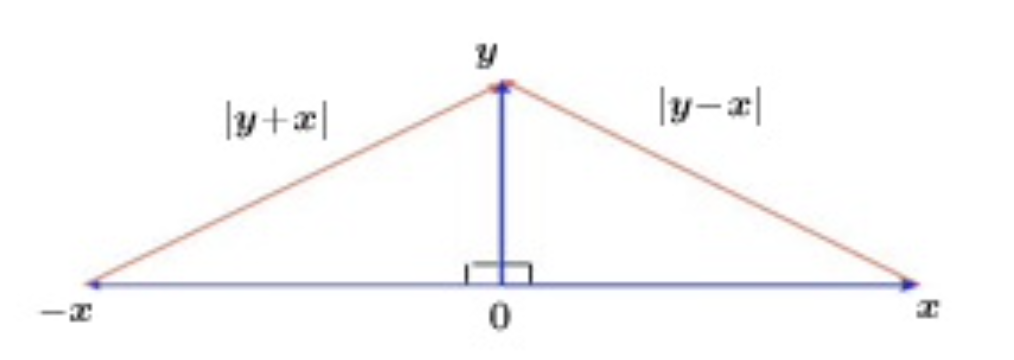
\includegraphics[scale=0.5]{p1}
\end{figure}

\definition[orthogonal projection]
The \ti{orthogonal projection} $\hat{\vy}$ of $\vy$ on any non-zero $\vx$ is a scalar multiple of $\vx$ and the \ti{residual vector} $\vy - \hat{\vy}$ is orthogonal to $\vx$:
\begin{equation}
	\begin{cases}
		\hat{\vy} = t\vx \quad \text{for some $t \in \real$} \\
		\vy - \hat{\vy} \perp \vx
	\end{cases}
\end{equation}
\begin{figure}[H]
	\centering
	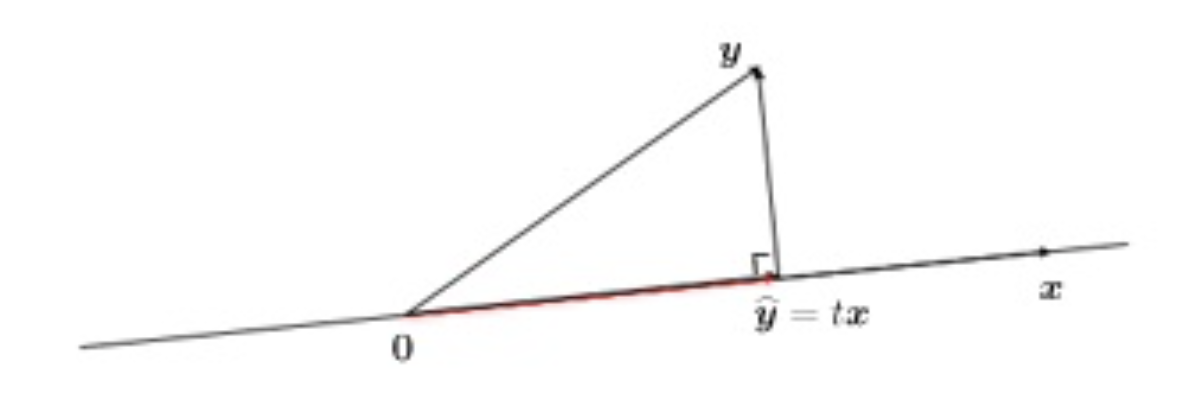
\includegraphics[scale=0.5]{p2}
\end{figure}
\remark
As follows.
\begin{enumerate}
	\item Then $\vx \cdot (\vy - t\vx) = 0$ and $t = \frac{\vx \cdot \vy}{|\vx|^2}$.
	\item Let $\theta$ be the angle described by $\vx$ and $\vy$. Then $\cos \theta = sign(\vx \cdot \vy) \frac{|\hat{\vy}|}{|\vy|} = \frac{\vx \cdot \vy}{|\vx||\vy|}$ 
\end{enumerate}

\property[Pythagorean Theorem]
\begin{equation}
	|\vy|^2 = |\hat{\vy} + (\vy - \hat{\vy})|^2 = |\hat{\vy}|^2 + |\vy - \hat{\vy}|^2
\end{equation}

\property[Cauchy-Schwarz inequalities]
As follows.
\begin{enumerate}
	\item $|\hat{\vy}| \leq |\vy|$ w.eq. iff $\vy = \hat{\vy}$
	\item $|\vx \cdot \vy| \leq |\vx||\vy|$ w.eq. iff $\vy = t\vx$ for $t \in \real$
	\item $|\cos \theta(\vx, \vy)| \leq 1$ w.eq. iff $\vy = t\vx$ for $t \in \real$
\end{enumerate}

\property[Triangle Inequality]
\begin{equation}
	|\vx + \vy| \leq |\vx| + |\vy| \quad \text{w.eq. iff $\vy = t\vx$ for $t > 0$}
\end{equation}

\subsection{The Natural Geometry of Random Variables}
\definition[L2 space]
By definition, $L$ is the vector space of real-valued random variables. We move to the particular \blue{sub-space of $L$} where the natural geometry of $\real^n$ has been reinvested in the random variables.
\begin{equation}
	L2 = \{X \in L |EX^2 < \infty\}
\end{equation}
In L2 we define 
\begin{enumerate}
	\item \tb{inner product} $\langle X, Y \rangle = EXY$
	\item \tb{length (norm)} $\norm{X} = \sqrt{\langle X, X \rangle} = \sqrt{EX^2}$
	\item \tb{distance (metric)} $d(X, Y) = \norm{Y - X} = \sqrt{E(Y - X)^2}$
\end{enumerate}

\subsubsection{Markov \& Chebyshev}

\theorem[Markov's Inequality]
For any $Z \geq 0, t \geq 0$ and non-decreasing $g: [0, \infty) \rightarrow [0, \infty)$, we have
\begin{equation}
	P(Z \geq t) \leq \frac{Eg(Z)}{g(t)} \quad \forall t \text{ s.t. } g(t) > 0
\end{equation}
\begin{proof}
\begin{align}
	g(t)I(Z\geq t) &\leq g(Z) \\
	g(t)P(Z \geq t) &\leq Eg(Z) \tag{applying $E$ to both sides} \\
	P(Z \geq t) &\leq \frac{Eg(Z)}{g(t)}
\end{align}
\end{proof}

\noindent Consider an arbitrary random variable $X$ in $L2$ with $\mu = EX$ and $\sigma^2 = E(X - \mu)^2$ and let $Z = |X - \mu|$ and $g(t) = \epsilon^2$ to get
\corollary[Chebyshev I] For any $X \in L_2, \epsilon > 0$, we have
\begin{equation}
	P(|X - \mu| \geq \epsilon) \leq \frac{\sigma^2}{\epsilon^2}
\end{equation}
Or take $Z = \frac{|X - \mu|}{\sigma}$ and $g(t) = k^2$ to find

\corollary[Chebyshev II]
For any $X \in L_2, k > 0$, we have
\begin{equation}
	P\left( \frac{|X - \mu|}{\sigma} > k \right) \leq \frac{1}{k^2}
\end{equation}

\corollary[Markov's Equality]
\begin{equation}
	E|X| = 0 \iff X \overset{wP1} = 0
\end{equation}

\subsubsection{The Geometry of $L_2$}
\definition[orthogonality]
\begin{equation}
	X \perp Y \iff \norm{Y - X} = \norm{Y + X} \iff \langle X, Y \rangle = EXY = 0
\end{equation}


\definition[orthogonal projection]
\begin{equation}
	\begin{cases}
		\hat{Y} = tX \quad \text{for some $t \in \real$} \\
		Y - \hat{Y} \perp X
	\end{cases}
\end{equation}

\remark
\begin{enumerate}
	\item Then $E(Y - tX) X = 0$ and $t = \frac{EXY}{EX^2}$ provided $EX^2 > 0$.
	\item $\cos \theta(X,Y) = sign(EXY)\frac{\norm{\hat{Y}}}{\norm{Y}} = \frac{EXY}{\sqrt{EX^2EY^2}}$
\end{enumerate}


\property[Pythagorean Theorem]
\begin{equation}
	\norm{Y}^2 = \norm{\hat{Y} + ( Y - \hat{Y})}^2 = \norm{\hat{Y}}^2 + \norm{Y - \hat{Y}}^2
\end{equation}

\property[Cauchy-Schwarz inequalities]
As follows.
\begin{enumerate}
	\item $\norm{\hat{Y}} \leq \norm{Y}$ w.eq. iff $Y \overset{wP1}{=} \hat{Y}$
	\item $(EXY)^2 \leq EX^2Y^2$ w.eq. iff $Y \overset{wP1}{=} tX$ for $t \in \real$
	\item $|\cos \theta(X, Y)| \leq 1$ w.eq. iff $Y = tX$ for $t \in \real$
\end{enumerate}

\property[Triangle Inequality]
\begin{equation}
	\norm{X + Y} \leq \norm{X} + \norm{Y} \quad \text{w.eq. iff $Y \overset{wP1}{=} tX$ for $t > 0$}
\end{equation}

\subsection{Covariance \& Correlation}
\definition[centred random variables] We define \ti{centred} version of random variable $X$ as 
$$\dot{X} = X - EX$$
The expected value of any centred random variables is zero:
$$E\dot{X} = 0$$
\remark
\begin{itemize}
	\item Variance is a quadratic operation instead of a linear one
	\item It is the inner product of the two centred variables:
	\begin{equation}
		cov(X, Y) := E\dot{X}\dot{Y} = E(X-EX)(Y-EY)
	\end{equation}
\end{itemize}

\definition[correlation coefficient]
We define the \ti{correlation coefficient} of $X$ and $Y$ to be the \ti{cosine of the angle} between the centred $X$ and $Y$
\begin{equation}
	\rho(X, Y):= \cos \theta(\dot{X}, \dot{Y}) = \frac{cov(X, Y)}{\sigma(X)\sigma(Y)}
\end{equation} 


\property[Cauchy-Schwarz inequalities]
As follows.
\begin{enumerate}
	\item $|cov(X, Y)| \leq \sqrt{varXvarY}$ w.eq. iff $Y \overset{wP1}{=} \alpha + \beta X$
	\item $|\rho(X,Y)| \leq 1$ w.eq. iff $Y \overset{wP1}{=} \alpha + \beta X$ 
\end{enumerate}

\subsection{Simple Linear Model}
\proposition Given any two real-valued r.v.s $X$ and $Y$, in $L_2$ there exist unique scalars $\alpha$ and $\beta$ and a unique r.v. $Z$ s.t.
\begin{equation}
	Y = \alpha + \beta X + Z \quad \text{w. $EZ = 0 = \rho(Z, X)$}
\end{equation}

\remark
We call $Z = Y - \alpha - \beta X$ a \ti{residual} variable.

\begin{figure}[H]
	\centering
	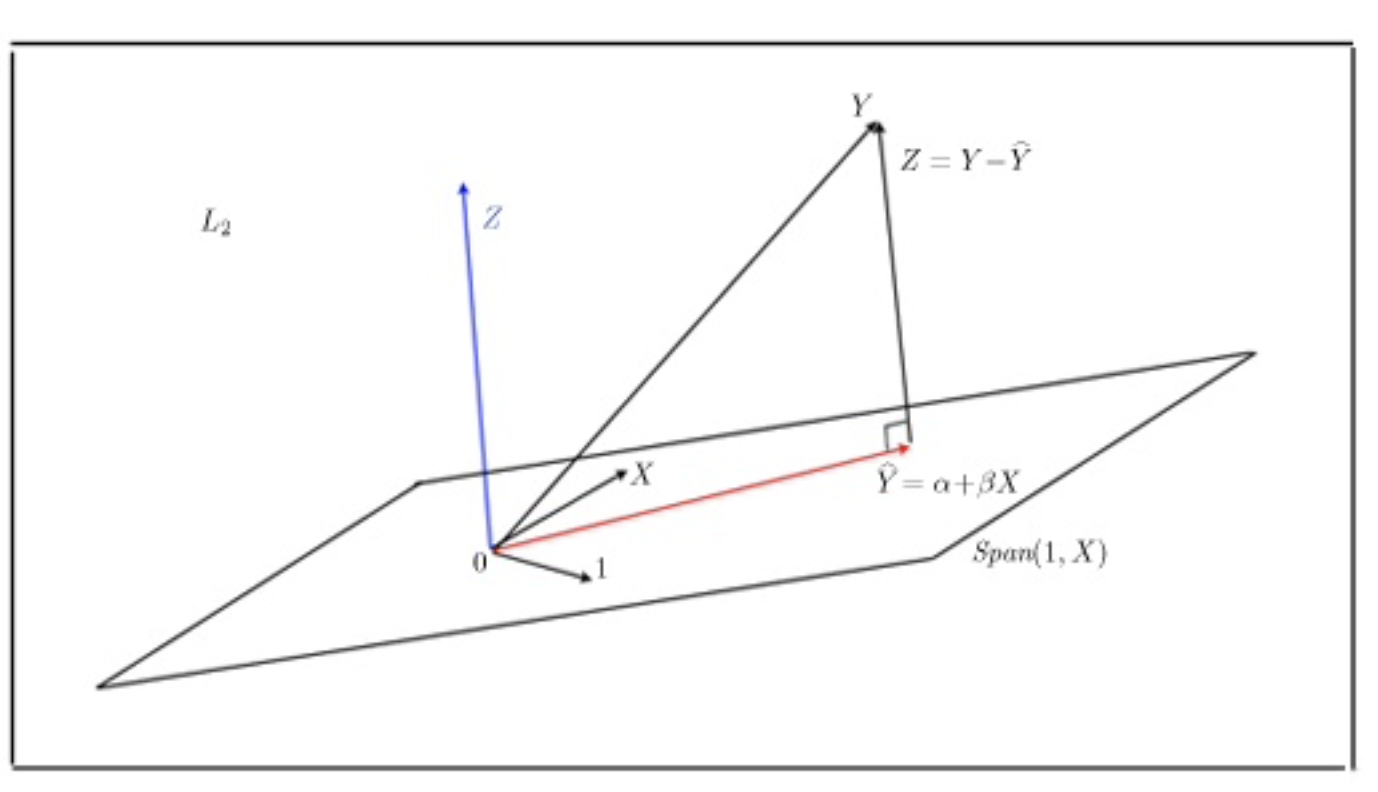
\includegraphics[scale=0.5]{p3}
\end{figure}

\corollary
\begin{equation}
\norm{Y - \alpha - \beta X} \leq \norm{Y - s - tX} \quad \text{w. eq. iff $s=\alpha, t = \beta$}
\end{equation}

\property[Pythagorean expression]
\begin{align}
	\norm{Y}^2 &= \norm{\alpha + \beta X}^2 + \norm{Z}^2 \\
	\implies varY &= var(\alpha + \beta X) + varZ \\
	&= \underbrace{\beta^2varX}_{cov(X,Y) = \beta varX} + varZ \\
	&= \rho(X, Y)^2 varY + varZ \\
	\implies \norm{Z}^2 &= varZ = (1 - \rho(X,Y)^2)varY \\
	\implies \frac{\norm{Y - \alpha - \beta X}}{\norm{Y - EY}} &= \frac{\sigma(Z)}{\sigma(Y)} = \sqrt{1 - \rho(X, Y)^2} \leq 1 \label{important}
\end{align}

\remark
(Equation \ref{important}) tells us the ratio of two physical distances: from $Y$ to $\hat{Y} = \alpha + \beta$ and from $Y$ to its own mean value. It will be strictly less than $1$ if $\rho(X, Y)$ is not trivial, which means $\hat{Y}$, a linear transformation of a random variable, can easily do better than a single real value.

\subsection{General Linear Model}
A \ti{$L_2$ prediction space} is any closed vector subspace $\mc{W} \subseteq L_2$, of r.v.s that contains the constants:
$$1 \in \mc{W} \overset{closed}{\subseteq} L_2$$ The best predictor of $Y$ in $\mc{W}$ is the unique element $\hat{Y}$ that is closest to $Y$.

\begin{figure}[H]
	\centering
	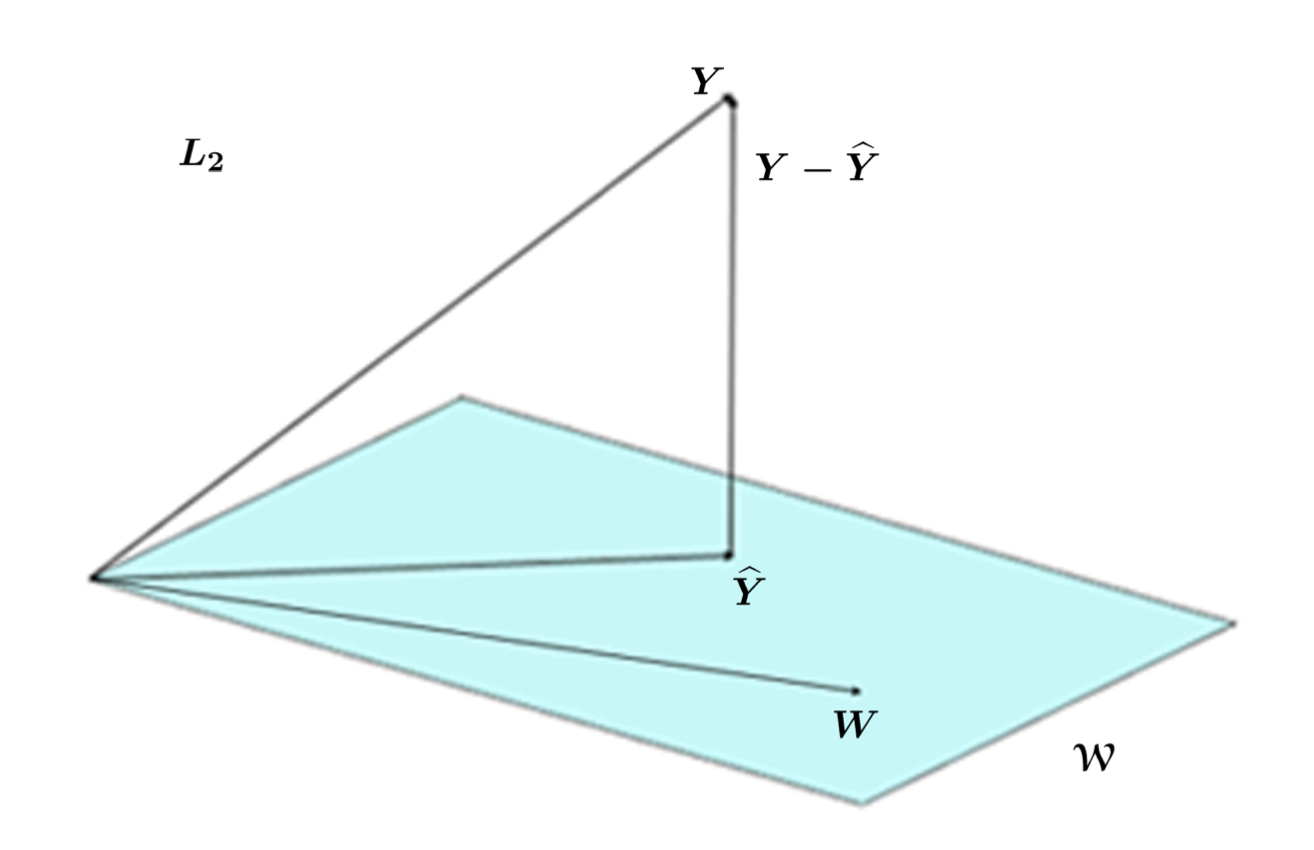
\includegraphics[scale=0.5]{p4}
\end{figure}
\noindent The \ti{orthogonal complement} of $\mc{W}$ is the vector subspace $\mc{W}^\perp$, of all r.v.s that are orthogonal to everything in $\mc{W}$ itself:
\begin{equation}
	\mc{W}^\perp = \{V \in L_2 | EVW = 0 \quad \forall W \in \mc{W}
\end{equation}
It is clear that $\mc{W} \cap \mc{W}^\perp = \{0\}$.

\definition[orthogonal projection]
The \ti{orthogonal projection} of $Y$ on $\mc{W}$, denoted $\hat{Y} = op(Y|\mc{W})$, is the random variable $\hat{Y}$ s.t.
$$\hat{Y} \in \mc{W} \quad \text{and} \quad Y - \hat{Y} \in \mc{W}^\perp$$

\proposition[orthogonal projection and minimum distance]
\begin{equation}
	\hat{Y} = op(Y|\mc{W}) \iff \norm{Y - \hat{Y}} = \inf_{W \in \mc{W}} \norm{Y - W}
\end{equation}

\proposition[general linear model]
For any $Y \in L_2$ and $1 \in \mc{W} \subseteq L_2$, there are unique $\hat{Y} \in \mc{W}$ and $Z$ s.t.
$$Y = \hat{Y} + Z \quad w. \quad EZ = 0 = \rho(Z, W) \quad \forall W \in \mc{W}$$

\proposition[maximum correlated estimator]
$Y = \hat{Y} + Z$ with $\hat{Y} \in \mc{W}, Z \in \mc{W}^\perp$ iff 
$$\rho(\hat{Y}, Y) = \sup_{W \in \mc{W}} \rho(W, Y) \quad w. \quad EZ = 0 = \rho(Z, \hat{Y})$$









\end{document}
